% !TeX spellcheck = en_US

\pdfminorversion=4 % for acroread
\documentclass[aspectratio=169,t,xcolor={usenames,dvipsnames}]{beamer}
%\documentclass[t,handout,xcolor={usenames,dvipsnames}]{beamer}
\usepackage{../beamerstyle}
\usepackage{dsfont}
\usepackage{bm}
\usepackage[english]{babel}
\usepackage[utf8]{inputenc}
\usepackage{graphicx}
\usepackage{algorithm}
\usepackage[ruled,vlined,algo2e,linesnumbered]{algorithm2e}
%\usepackage[boxed,vlined]{algorithm2e}
\usepackage{hyperref}
\usepackage{booktabs}
\usepackage{mathtools}

\usepackage{amsmath,amssymb}
\usepackage{listings}
\lstset{frame=lines,framesep=3pt,numbers=left,numberblanklines=false,basicstyle=\ttfamily\small}

\usepackage{subfig}
\usepackage{multicol}
%\usepackage{appendixnumberbeamer}
%
\usepackage{tcolorbox}

\usepackage{pgfplots}
\usepackage{tikz}
\usetikzlibrary{trees} 
\usetikzlibrary{shapes.geometric}
\usetikzlibrary{positioning,shapes,shadows,arrows,calc,mindmap}
\usetikzlibrary{positioning,fadings,through}
\usetikzlibrary{decorations.pathreplacing}
\usetikzlibrary{intersections}
\usetikzlibrary{positioning,fit,calc,shadows,backgrounds}
\pgfdeclarelayer{background}
\pgfdeclarelayer{foreground}
\pgfsetlayers{background,main,foreground}
\tikzstyle{activity}=[rectangle, draw=black, rounded corners, text centered, text width=8em]
\tikzstyle{data}=[rectangle, draw=black, text centered, text width=8em]
\tikzstyle{myarrow}=[->, thick, draw=black]

% Define the layers to draw the diagram
\pgfdeclarelayer{background}
\pgfdeclarelayer{foreground}
\pgfsetlayers{background,main,foreground}

%\usepackage{listings}
%\lstset{numbers=left,
%  showstringspaces=false,
%  frame={tb},
%  captionpos=b,
%  lineskip=0pt,
%  basicstyle=\ttfamily,
%%  extendedchars=true,
%  stepnumber=1,
%  numberstyle=\small,
%  xleftmargin=1em,
%  breaklines
%}

 
\definecolor{blue}{RGB}{0, 74, 153}

\usetheme{Boadilla}
%\useinnertheme{rectangles}
\usecolortheme{whale}
\setbeamercolor{alerted text}{fg=blue}
\useoutertheme{infolines}
\setbeamertemplate{navigation symbols}{\vspace{-5pt}} % to lower the logo
\setbeamercolor{date in head/foot}{bg=blue} % blue
\setbeamercolor{date in head/foot}{fg=white}
\setbeamercolor{author in head/foot}{bg=blue} %blue
\setbeamercolor{title in head/foot}{bg=blue} % blue
\setbeamercolor{title}{fg=white, bg=blue}
\setbeamercolor{block title}{fg=white,bg=blue}
\setbeamercolor{block body}{bg=blue!10}
\setbeamercolor{frametitle}{fg=white, bg=blue}
\setbeamercovered{invisible}

\makeatletter
\setbeamertemplate{footline}
{
  \leavevmode%
  \hbox{%
  \begin{beamercolorbox}[wd=.333333\paperwidth,ht=2.25ex,dp=1ex,center]{author in head/foot}%
    \usebeamerfont{author in head/foot}\insertshortauthor
  \end{beamercolorbox}%
  \begin{beamercolorbox}[wd=.333333\paperwidth,ht=2.25ex,dp=1ex,center]{title in head/foot}%
    \usebeamerfont{title in head/foot}\insertshorttitle
  \end{beamercolorbox}%
  \begin{beamercolorbox}[wd=.333333\paperwidth,ht=2.25ex,dp=1ex,right]{date in head/foot}%
    \usebeamerfont{date in head/foot}Week \@week, Topic \@topicnumber, Slide \insertframenumber{}\hspace*{2em}
%    \insertframenumber\hspace*{2ex} 
  \end{beamercolorbox}}%
  \vskip0pt%
}

\newcommand{\@week}{0}
\newcommand{\@topicnumber}{0}
\newcommand{\week}[1]{\renewcommand{\@week}{#1}}
\newcommand{\topicnumber}[1]{\renewcommand{\@topicnumber}{#1}}

\makeatother

%\pgfdeclareimage[height=1.2cm]{automl}{images/logos/automl.png}
%\pgfdeclareimage[height=1.2cm]{freiburg}{images/logos/freiburg}

%\logo{\pgfuseimage{freiburg}}

\input{../latex_main/macros}






\title[AutoML: PBT]{AutoML: Dynamic Configuration \& Learning}
\subtitle{Population-based Training}
\author[Marius Lindauer]{Bernd Bischl \and Frank Hutter \and Lars Kotthoff\newline \and \underline{Marius Lindauer} \and Joaquin Vanschoren}
\institute{}
\date{}
\week{11}
\topicnumber{4}



% \AtBeginSection[] % Do nothing for \section*
% {
%   \begin{frame}{Outline}
%     \bigskip
%     \vfill
%     \tableofcontents[currentsection]
%   \end{frame}
% }

\begin{document}
	
	\maketitle
	
	
%----------------------------------------------------------------------
%----------------------------------------------------------------------
\begin{frame}[c]{On-the-fly Adaption}

\begin{itemize}
	\item Dynamic algorithm configuration assumes that we have access to\\ a \alert{representative learning environment} in an \alert{offline learning phase}
	\pause
	\item What if we don't access to such an env or don't have to time for offline learning?
	\pause
	\bigskip
	\item[$\leadsto$] Try to figure out best hyperparameter settings on the fly
\end{itemize}

\end{frame}
%----------------------------------------------------------------------
%----------------------------------------------------------------------
\begin{frame}[c]{Massively parallelized Random Search}

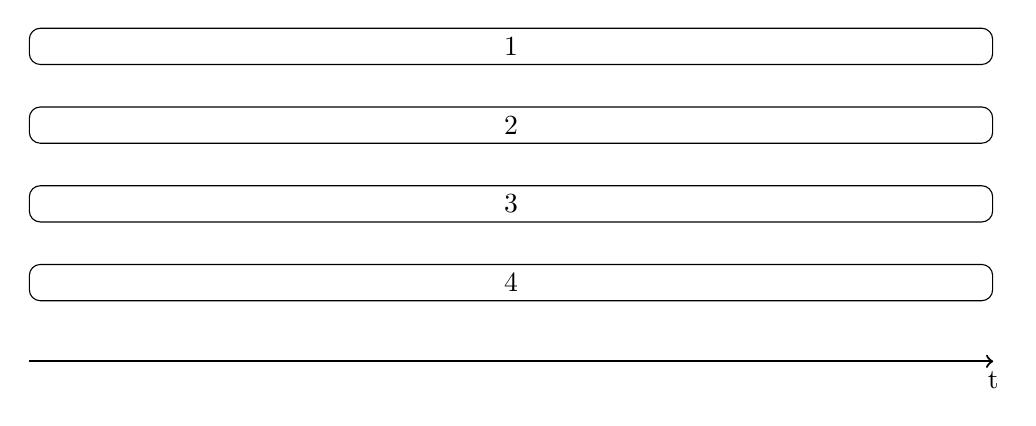
\begin{tikzpicture}[node distance=2.1cm]
%PreProcessing

\node (l1) [activity, text width=12cm] {$\confI{1}$};
\node (l2) [activity, below of=l1, node distance=1cm, text width=12cm] {$\confI{2}$};
\node (l3) [activity, below of=l2, node distance=1cm, text width=12cm] {$\confI{3}$};
\node (l4) [activity, below of=l3, node distance=1cm, text width=12cm] {$\confI{4}$};

\draw[myarrow] ($(l4.west)+(0.0, -1.0)$) -- ($(l4.east)+(0.0, -1.0)$) node[below] {t};

\end{tikzpicture}

\bigskip
\begin{itemize}
	\item Sample many hyperparameter configurations $\confI{i}$ and evaluate them all in parallel
	\pause
	\item Pure exploration on a large population of configurations
	\pause
	\item No dynamic adaptation
\end{itemize}

\end{frame}
%----------------------------------------------------------------------
%----------------------------------------------------------------------
\begin{frame}[c]{Population-based Training \litw{\href{https://arxiv.org/pdf/1711.09846.pdf}{Jaderberg et al. 2017}}}

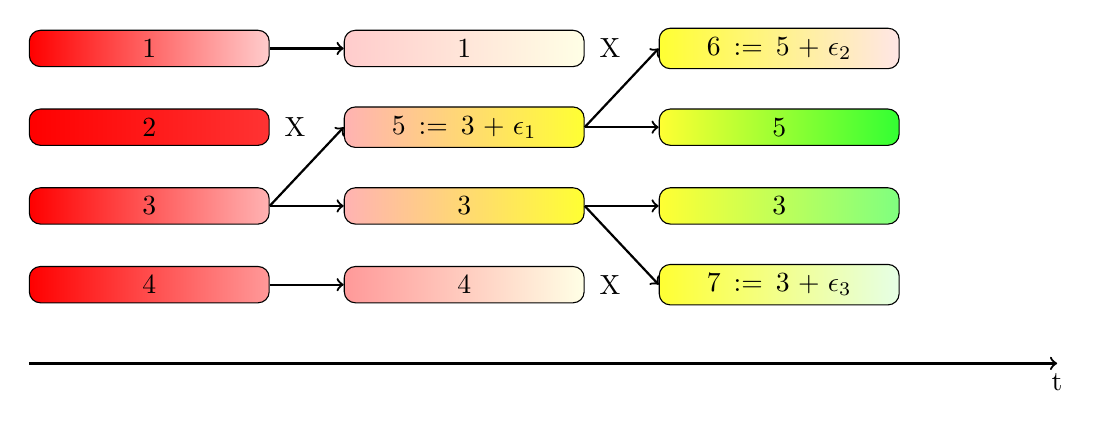
\begin{tikzpicture}[node distance=2.1cm]
%PreProcessing

\node (l1) [activity, left color=red!100, right color=red!20] {$\confI{1}$};
\node (l2) [activity, left color=red!100, right color=red!80, below of=l1, node distance=1cm] {$\confI{2}$};
\node (l3) [activity, left color=red!100, right color=red!30, below of=l2, node distance=1cm] {$\confI{3}$};
\node (l4) [activity, left color=red!100, right color=red!40, below of=l3, node distance=1cm] {$\confI{4}$};

\draw[myarrow] ($(l4.west)+(0.0, -1.0)$) -- ($(l4.east)+(10.0, -1.0)$) node[below] {t};

\pause

\node (l12) [activity, right of=l1, left color=red!20, right color=yellow!10, node distance=4cm] {$\confI{1}$};
\node (l22X) [right of=l2, node distance=1.85cm]{X};
\node (l22) [activity, left color=red!30, right color=yellow!80, right of=l2, node distance=4cm]{$\confI{5} := \confI{3} + \epsilon_1$};
\node (l32) [activity, left color=red!30, right color=yellow!80, right of=l3, node distance=4cm] {$\confI{3}$};
\node (l42) [activity, left color=red!40, right color=yellow!10, right of=l4, node distance=4cm] {$\confI{4}$};

\draw[myarrow] (l1.east) -- (l12.west);
\draw[myarrow] (l3.east) -- (l22.west);
\draw[myarrow] (l3.east) -- (l32.west);
\draw[myarrow] (l4.east) -- (l42.west);

\pause

\node (l13X) [right of=l12, node distance=1.85cm]{X};
\node (l13) [activity, left color=yellow!80, right color=red!10, right of=l12, node distance=4cm] {$\confI{6} := \confI{5} + \epsilon_2$};
\node (l23) [activity, left color=yellow!80, right color=green!80, right of=l22, node distance=4cm]{$\confI{5}$};
\node (l33) [activity, left color=yellow!80, right color=green!50, right of=l32, node distance=4cm] {$\confI{3}$};
\node (l43X) [right of=l42, node distance=1.85cm]{X};
\node (l43) [activity, left color=yellow!80, right color=green!10, right of=l42, node distance=4cm] {$\confI{7} := \confI{3} + \epsilon_3$};

\draw[myarrow] (l22.east) -- (l13.west);
\draw[myarrow] (l22.east) -- (l23.west);
\draw[myarrow] (l32.east) -- (l33.west);
\draw[myarrow] (l32.east) -- (l43.west);

\end{tikzpicture}

\begin{itemize}
	\item The color indicates the performance over time
\end{itemize}

\end{frame}
%----------------------------------------------------------------------
%----------------------------------------------------------------------
\begin{frame}[c]{Population-based Training \litw{\href{https://arxiv.org/pdf/1711.09846.pdf}{Jaderberg et al. 2017}; \href{https://arxiv.org/pdf/2002.04225.pdf}{Liang et al. 2020}}}

General workflow of PBT:

\begin{enumerate}
	\item Sample initial population
	\begin{itemize}
		\item Each population member is a combination of hyperparameter setting $\conf$ and (partially trained) model
	\end{itemize}
	\pause
	\item Train population for a bit 
	\pause
	\item Tournament selection to drop poorly performing population members
	\pause
	\item Use mutation (and cross-over) to generate off-springs
	\begin{itemize}
		\item Change the hyperparameter settings, but inherits the partially trained model (+ pertubation)
	\end{itemize}
	\pause
	\item[$\leadsto$] New population consists of so-far best performing ones and new off-springs
	\pause
	\item Go to 2.
\end{enumerate}


\end{frame}
%----------------------------------------------------------------------
%----------------------------------------------------------------------
\begin{frame}[c]{Properties of Population-based Training (PBT)}

\begin{itemize}
	\item PBT returns an already trained model (e.g., DNN or RL policy)
	\bigskip
	\pause
	\item PBT uses evolutionary computing to determine well-performing hyperparameter settings
	\bigskip
	\pause
	\item Since hyperparameter settings changes while training the models,\\ PBT relates to dynamic algorithm configuration
	\bigskip
	\pause
	\item Since each population member (i.e., model) can be trained independently,\\ PBT can be efficiently parallelized
	\begin{itemize}
		\item[$\leadsto$] Drawback: requires substantial parallel compute resources
	\end{itemize}
\end{itemize}

\end{frame}
%----------------------------------------------------------------------
%----------------------------------------------------------------------
\begin{frame}[c]{Combining Population-based Training and Bayesian Optimization}

\begin{itemize}
	\item Bayesian Optimization (BO) is well known for its sample efficiency
	\pause
	\medskip
	\item \alert{Idea:} Can we use BO to guide PBT? 
	\pause
	\medskip
	\item[$\leadsto$] Less parallel compute resources are required(?)
	\pause
	\medskip
	\item[$\leadsto$] Scales better to higher dimensional spaces(?)
\end{itemize}

\end{frame}
%----------------------------------------------------------------------
%----------------------------------------------------------------------
\begin{frame}[c]{PBT + BO: Outline}

\begin{enumerate}
	\item Sample initial population
	\begin{itemize}
		\item Each population member is a combination of hyperparameter setting $\conf$ and (partially trained) model
	\end{itemize}
	\item Train population for a bit 
	\item Tournament selection to drop poorly performing population members
	\item Use \alert{Bayesian optimization} to select new hyperparameter settings
	\begin{itemize}
		\item Change the hyperparameter settings, but inherits the partially trained model (+ pertubation)
	\end{itemize}
	\item[$\leadsto$] New population consists of so-far best performing ones and new off-springs
	\item Go to 2.
\end{enumerate}


\end{frame}
%----------------------------------------------------------------------
%----------------------------------------------------------------------
\begin{frame}[c]{PBT  + BO: Parallel Evaluation}

\begin{itemize}
	\item \alert{Challenge I}: PBT runs in parallel asynchronously
	\pause
	\medskip
	\item[$\leadsto$] BO has to take into account that other hyperparameter settings are being evaluated already
	\pause 
	\medskip
	\item Several ideas on how to parallelize BO
	\begin{itemize}
		\pause
		\smallskip
		\item Randomize the model training or optimization of the acquisition function
		\pause
		\smallskip
		\item Thompson sampling to use only a single explanation of the data\newline (in proportion to its likelihood)
		\pause
		\smallskip
		\item Hallucinate performance of other hyperparameter settings in optimistically, pessimistically or in expectation of the current surrogate model
	\end{itemize}
	
\end{itemize}

\end{frame}
%----------------------------------------------------------------------
%----------------------------------------------------------------------
\begin{frame}[c]{PBT  + BO: Parallel Evaluation \litw{\href{https://arxiv.org/pdf/2002.02518.pdf}{Parker-Holder et al. 2020}}}

\begin{itemize}
	\item \alert{Challenge II}: The cost depends on the previous $\confI{1}, \confI{2}. \ldots, \confI{t-1}$
	\pause
	\medskip
	\item BO-Surrogate model predicts the cost improvement over time:
\end{itemize}

\begin{equation}
\cost_{\text{PBT}}^{(t)}(\conf)= \frac{\cost^{(t)}(\conf) - \cost^{(t-1)}(\conf)}{\Delta t}\nonumber
\end{equation}

where $\cost^{(t)}(\conf)$ is the cost for a given hyperparameter setting at time step $t$.

\bigskip
\pause
\begin{itemize}
	\item Remark: Also add $\cost^{(t-1)}$ as an input to the BO-surrogate model to\\ ease the task of predicting the improvement
\end{itemize}

\end{frame}
%----------------------------------------------------------------------

\end{document}